
\documentclass[../main.tex]{subfiles}
\begin{document}
\section{Chip Summary}
\label{sec:Chip-summary}
The CHIPS architecture uses the Mie Fujitsu 55nm LP process. Figure ?? shows a photograph of the chip die (chiplets and support structures are highlighted). Each chiplet can operate at 250Mhz core clock frequency, and with the support structure, the core clock frequency reduces to 50Mhz. All chiplets and support structures are projected to work at the typical typical corner, at 0.8-V digital supply voltage (VDD) and 40 degrees Celsius. 

%\begin{figure}
%    \centering
%   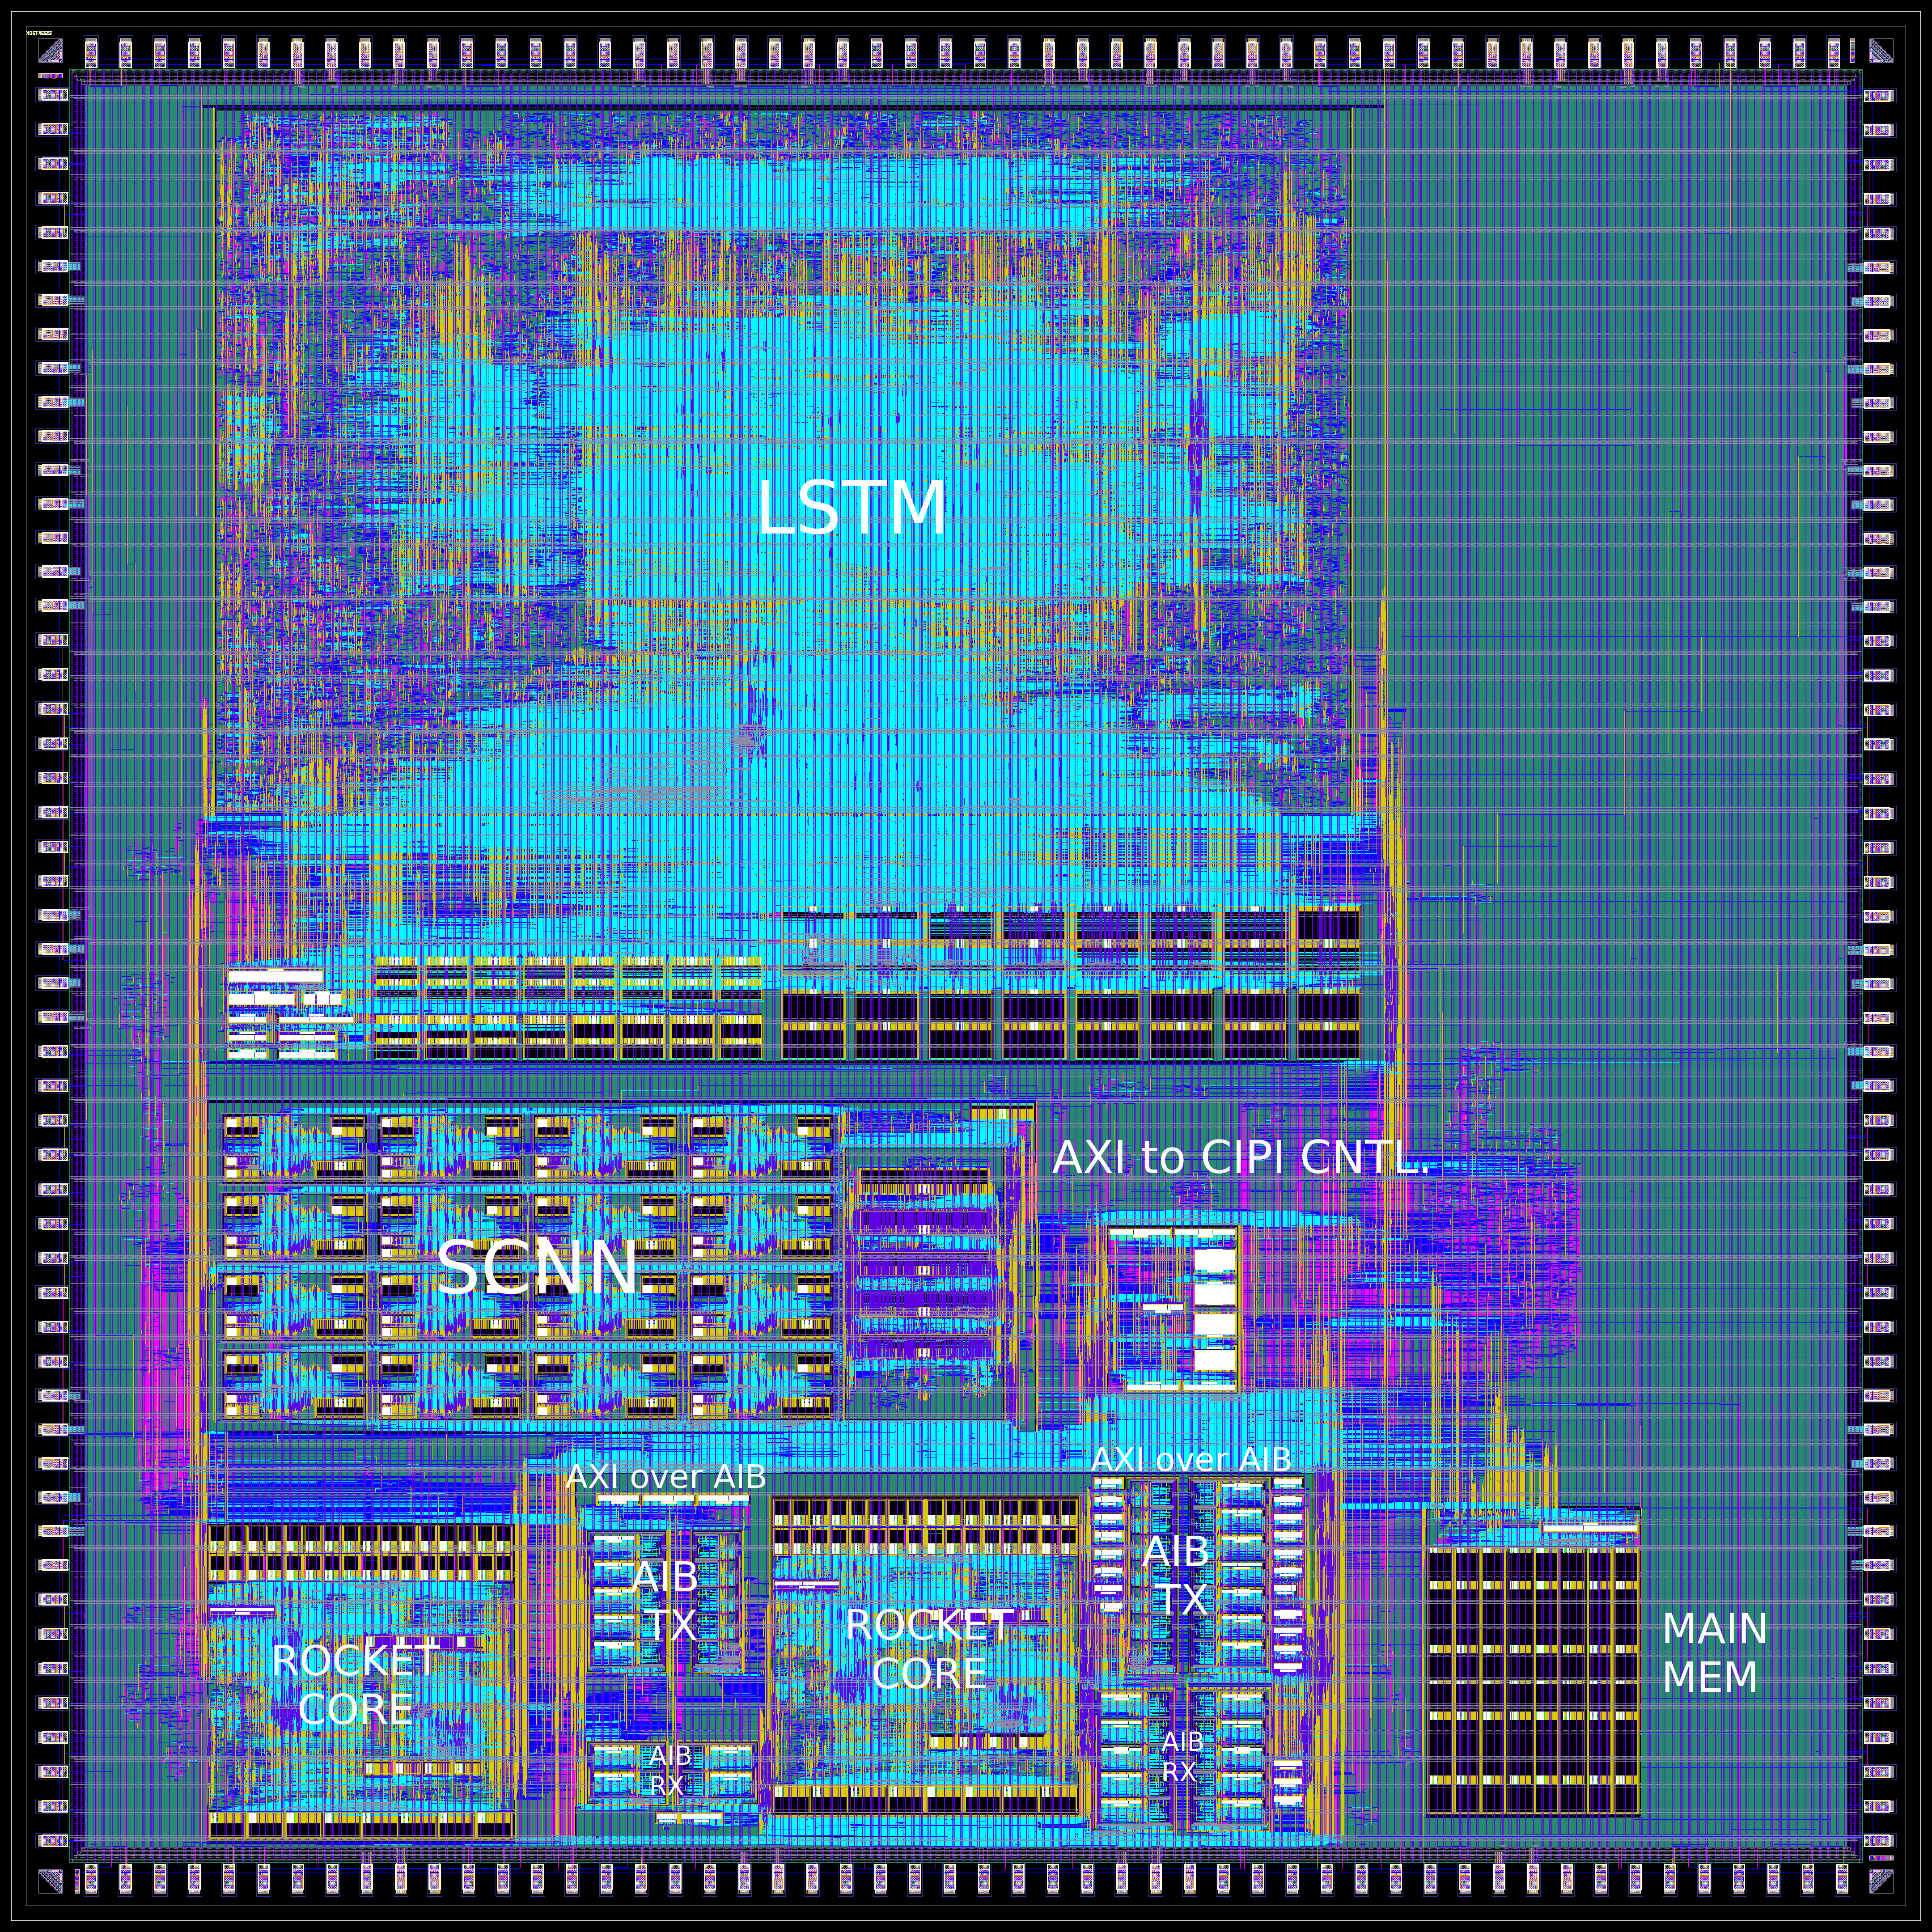
\includegraphics[scale=.06]{pngs/CHIPS-Layout.png}
%    \caption{CHIPS Layout [Provided by Steve Lipa]}
%    \label{fig:CHIPS-layout}
%\end{figure}

\end{document}